\section{Umsetzung}
\subsection{Technologie und Plattform}
In der Problembeschreibung zu dieser Arbeit wurden die Anforderungen an eine SmartHome Lösung diskutiert. In der anschliessenden Marktanalyse wurde openHAB als Grundlage zur Umsetzung unseres Projekts evaluiert. OpenHAB erfüllt die geforderten Kritierien, wie Herstellerunabhängigkeit, Installierbarkeit und Flexibilität. Cloudseitig wird MS Azure Cloud zur Persistierung von Events verwendet.


\subsection{openHAB Konfiguration}
Items, Rules, Sitemaps und Persitence Strategies werden in openHAB in einer eigens dafür entwickelten DSL beschrieben. Für alle diese Bereiche werden Konfigurationsdateien im entsprechenden Unterverzeichnis des openHAB Konfigurationsordner abgelegt. Änderungen an den Konfigurationsdateien werden von openHAB zur Laufzeit sofort erkannt und berücksichtigt. Nebst den genannten Bereichen existiert noch eine globale Konfigurationsdatei um beispielsweise IP-Adressen für Bindings einzutragen. Folgende Dateien sind für diese Arbeit relevant:

\begin{itemize}
	\item /configurations/*.cfg
	\item /configurations/items/*.items
	\item /configurations/rules/*.rules
	\item /configurations/sitemaps/*.sitemap
	\item /configurations/persistence/*.persist
	\item /configurations/transform/*.map
\end{itemize}

Anhand diesen Konfigurationen werden die User Cases modelliert.

\subsubsection{Konfiguration Überwachungskamera} 
Für die Überwachungskamera existiert kein entsprechendes Item. Stattdessen wird in der Sitemap ein Image-Element angezeigt, dessen URL auf das HTTP Snapshot Interface der Netzwerkkamera verweist.\\ \\
Das Bild wird dank dem Attribut \lstinline!visibility!  immer dann angezeigt, wenn das Item \lstinline!Alarm_activated! den Wert \lstinline!ON! hat. Das \lstinline!refresh! Interval bewirkt einen Reload des Bildes alle 200 Millisekunden.

\begin{lstlisting}[style=csharp, caption=demo.sitemap - Webcam Bild]
[...]
Image url="http://192.168.1.15/snapshot.jpg" refresh=200
visibility=[Alarm_activated==ON]
[...]
\end{lstlisting}




\subsubsection{Konfiguration Kontaktsensor} 
Der Kontaktsensor ist ein Use Case der in openHAB sehr oft vorkommt. Deshalb existiert ein Item Type «Contact» mit den beiden möglichen Werten OPEN und CLOSED. Das Homematic Binding liefert aber die Werte \lstinline!true! oder \lstinline!false! und kann deshalb nicht an ein Contact Item gebunden werden. Als Alternative haben wir ein String Item verwendet und mit Hilfe einer Transformation-Map \lstinline!false! mit «geschlossen» und \lstinline!true! mit «offen» übersetzt. Das Icon <contact> kann trotzdem noch verwendet werden. Allerdings wird nun nicht mehr automatisch das Icon für das offene bzw. geschlossene Fenster angezeigt, da openHAB den Basisnamen des Icons mit dem State konkateniert. Wir haben dementsprechend die Icons kopiert und ein File contact-false.png und contact-true.png im Ressourcen-Ordner hinterlegt.\\ \\
Auf der letzten Zeile werden die Bindingparameter für Homematic angegeben.\\ \lstinline!address=LEQ1469091! bezieht sich auf die Seriennummer des Kontaktsensors und\\ \lstinline!parameter=STATE! gibt an, welche Eigenschaft gebunden werden soll. \lstinline!channel=1! ist ein Defaultwert.

\begin{lstlisting}[style=csharp, caption=demo.items - Kontaktsensor]
[...]
String Window_Bedroom "Schlafzimmerfenster [MAP(window.map):%s]"
<contact> (OV_Windows, Windows)
{homematic="address=LEQ1469091,channel=1,parameter=STATE"}
[...]
\end{lstlisting}

In der Sitemap wird das Item in einem Text-Element referenziert. Weitere Attribute sind nicht notwendig.

\begin{lstlisting}[style=csharp, caption=demo.sitemap - Kontaktsensor]
[...]
Text item=Window_Bedroom
[...]
\end{lstlisting}

\subsubsection{Konfiguration Bewegungsmelder}
Der Bewegungsmelder ist ebenfalls von Homematic und wird in den Bindingparametern gleich referenziert wie beim Kontaktsensor. Der Bindingparameter \lstinline!MOTION! erhält einen boolschen Wert und muss mit Hilfe der Map \lstinline!motion.map! in einen benutzerfreundlichen String transformiert werden. Der Parameter \lstinline!ERROR! dient dem Sabotageschutz.\\ \\
Leider muss bei Homematic jeder Parameter einem eigenen Item zugeordnet werden. Deshalb haben wir ein drittes String-Item \lstinline!Motion_Summary! definiert, indem die Werte der beiden anderen Items zusammengefasst werden. 


\begin{lstlisting}[style=csharp, caption=demo.items - Bewegungsmelder Items]
[...]
String Motion_Livingroom "Bewegungsmelder [MAP(motion.map):%s]"
{homematic="address=LEQ0797607, channel=1, parameter=MOTION"}

String Motion_Livingroom_Sabotage "Sabotage"
{homematic="address=LEQ0797607, channel=1, parameter=ERROR"}

String Motion_Summary "Bewegungsmelder [%s]"
[...]
\end{lstlisting}

Die Ermittlung und Zuweisung des korrekten Wertes an das Item \lstinline!Motion_Summary! geschieht mit Hilfe der Rule \lstinline!Motion Aggregator!, die im nächsten Abschnitt erklärt wird.

\subsubsection{Rules}
Wie im Lösungskonzept beschrieben, werden Rules zur Automatisierung von Aktionen eingesetzt. Die Regeln können im File \lstinline!/etc/openhab/configurations/rules/demo.rules! definiert werden. \\\\
\textbf{Alarm} \\
In der Grafik \ref{fig:flowchartAlarm} wird der Ablauf der Alarm-Regel gezeigt. Im Wesentlichen geht es darum, beim Erkennen von Bewegung und offenem Fenster das Licht einzuschalten und die aufgenommenen Bilder der Webcam zu speichern. Dies soll jedoch nur geschehen, wenn der Alarm eingeschaltet ist.
\begin{figure}[H]
	\centering
		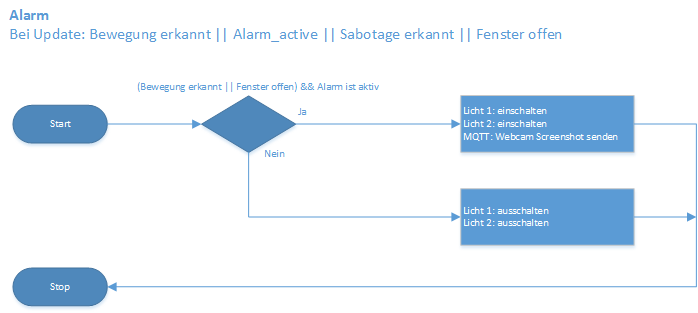
\includegraphics[scale=0.8]{report/img/RuleAlarm}
	\caption{Flowchart Alarm Rule}
	\label{fig:flowchartAlarm}
\end{figure}

Umgesetzt wird diese Flowchart durch folgenden Code. Diese Rules sind in der von openHAB selbst definierten DSL (Domain Specific Language) geschrieben.

\begin{lstlisting}[style=csharp, caption=demo.rules - Rule «Motion Aggregator»]
rule "Alarm"
	when Item Motion_Livingroom received update or
	     Item Motion_Livingroom_Sabotage received update or
	     Item Window_Bedroom received update
	then
	if(Motion_Livingroom.state == "true" ||
	   Window_Bedroom.state == "true") {
		sendCommand(Hue_1, ON)
		sendCommand(Hue_2, ON)
		sendMqttFile("openhab/blob",
					 "http://192.168.1.15/snapshot.jpg")
	} else {
		sendCommand(Hue_1, OFF)
		sendCommand(Hue_2, OFF)
	}
end
\end{lstlisting}

\textbf{Bewegungsmelder Aggregation} \\
Diese Regel definiert die verschiedenen Status, die der Bewegungsmelder haben kann. Durch diese Regel wird der aktuelle Status ermittelt und für das Item \lstinline!Motion_Summary! gesetzt. \\
Da der Bewegungsmelder Bewegungen und Sabotage erkennen kann (wenn die Halterung entfernt wird), ergeben sich vier mögliche Zustände: «Ruhig», «Bewegung erkannt», «Bewegung und Sabotage erkannt» und «Sabotage erkannt».\\
In der Abbildung \ref{fig:flowChartMotionAggregator} wird der Ablauf illustriert.

\begin{figure}[H]
	\centering
		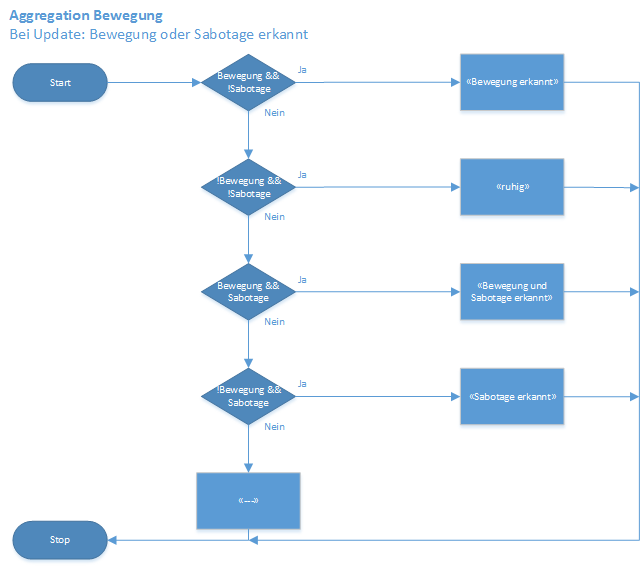
\includegraphics[scale=0.8]{report/img/RuleMotionAggregator}
	\caption{Flowchart Motion Aggregator Rule}
	\label{fig:flowChartMotionAggregator}
\end{figure}

Nachfolgend ist die Definition der Regel in der openhAB DSL beschrieben. Falls keiner der vier möglichen Zustände zutrifft, was nur in einem Fehlerfall möglich ist, wird «---» im Item \lstinline!Motion_Summary! angezeigt.

\begin{lstlisting}[style=csharp, caption=demo.rules - Rule «Motion Aggregator»]
rule "Motion Aggregator"
	when Item Motion_Livingroom received update or
	     Item Motion_Livingroom_Sabotage received update
	then
	if(Motion_Livingroom.state == "true" &&
	   Motion_Livingroom_Sabotage.state == "NO_ERROR") {
		postUpdate(Motion_Summary, "Bewegung erkannt")
	} else if(Motion_Livingroom.state == "false" && 
	          Motion_Livingroom_Sabotage.state == "NO_ERROR") {
		postUpdate(Motion_Summary, "ruhig")	
	} else if(Motion_Livingroom.state == "true" &&
	          Motion_Livingroom_Sabotage.state == "SABOTAGE") {
		postUpdate(Motion_Summary, "Bewegung und Sabotage!")
	} else if(Motion_Livingroom.state == "false" &&
	          Motion_Livingroom_Sabotage.state == "SABOTAGE")  {
		postUpdate(Motion_Summary, "Sabotage")
	} else {
		postUpdate(Motion_Summary, "---")
	}
end
\end{lstlisting}

\pagebreak


\subsection{Deploymentübersicht}

\subsubsection{Binding Azure}
\begin{figure}[H]
	\centering
		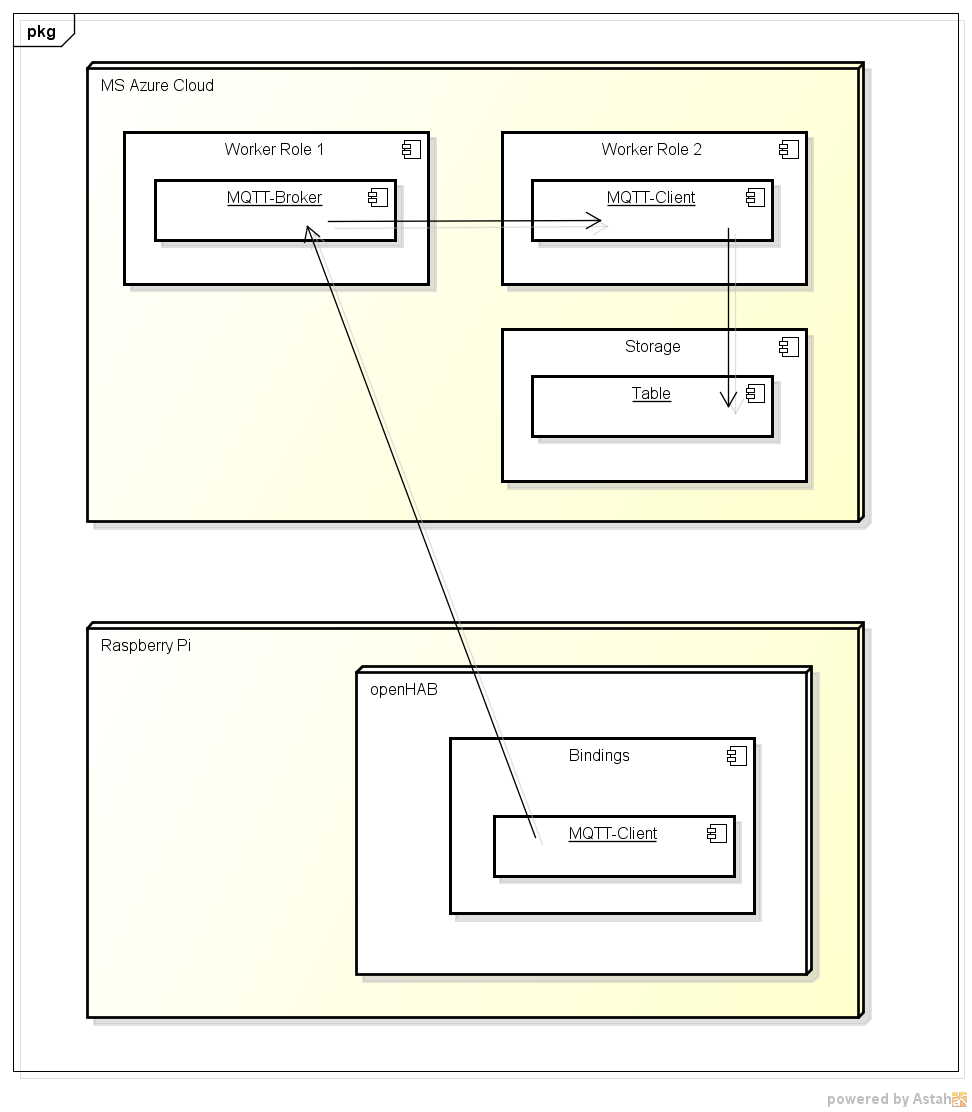
\includegraphics[scale=0.5]{report/img/deployment_binding_azure}
	\caption{Binding Azure Cloud}
	\label{fig:deploymentAzure}
\end{figure}

\subsection{MQTT} \label{sssec:mqtt}
MQTT steht für «Message Queue Telemetry Transport» und ist ein Nachrichten-Protokoll, das speziell für IOT-Anwendungen konzipiert wurde. Es setzt auf dem TCP/IP Stack auf und wird für den Nachrichtenaustausch zwischen verschiedenen, verteilten Maschinen verwendet. \\
Das Protokoll wurde speziell für Systeme designt, die über wenig Speicherplatz und kleiner Netzwerk-Bandbreite verfügen, was bei IOT-Anwendungen meist der Fall ist.

\subsubsection{Funktionsweise}
MQTT folgt dem Prinzip «Publish/Subscribe», sprich Clients können bestimmte Topics abonnieren. Wenn Messages auf dieses Topic gesendet werden, leitet der Broker diese an alle interessierten Clients weiter. \\
In Bezug auf erstellen von Topics agiert der Broker passiv. Das bedeutet, Clients können sich auf beliebigen, selber defnierte, Topics registrieren. Wenn aber niemand auf dieses Topic publiziert, wird der Client nie eine Message erhalten.

\begin{figure}[H]
	\centering
		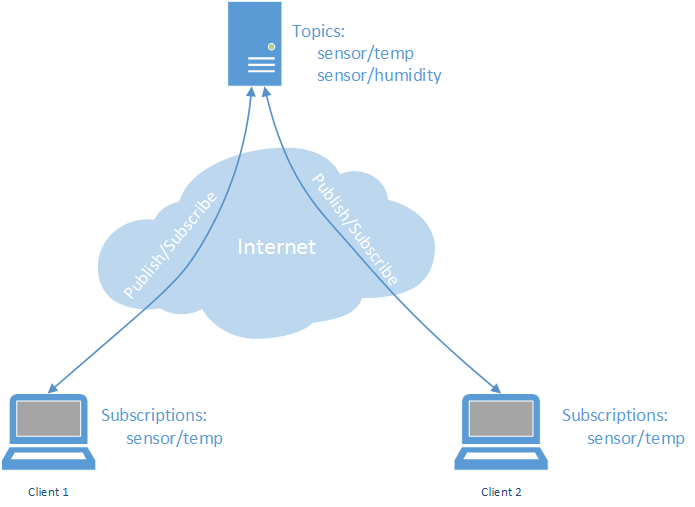
\includegraphics[scale=0.6]{report/img/mqttFunktionsweise}
	\caption{Funktionsweise MQTT}
	\label{fig:funktionsweiseMQTT}
\end{figure}

\subsubsection{Broker}

\textbf{Zertifizierungsstelle/Server-Zertifikat} \\
Da die MQTT-Verbindung verschlüsselt werden soll, müssen verschiedene Zertifikate erstellt werden. Das erstellte Server-Zertifikat muss von einer CA (Certification Authority) signiert werden. Da ein gültiges Zertifikat nicht entgeltlich erworben werden möchte, wird eine eigene Zertifizierungsstelle erstellt. OpenSSl bringt da alle nötigen Mittel für die Erzeugung eines CAs mit. Dies bringt den Nachteil mit, dass Computersysteme diesem Zertifikat nicht automatisch trauen, daher muss dann das Zertifkat von Hand dem Certificate Store als «Trusted Root Certification Authority» hinzugefügt werden. \\

Nachdem die Zertifizierungsstelle erfolgreich generiert wurde, kann das Server Zertifikat erstellt werden. Anschliessend muss dieses Server Zertifikat von der eben erstellten Zertifizierungsstelle signiert werden.

Da sowohl die Zertifizierungsstelle, als auch das Server-Zertifikat auf dem gleichen Computer erstellt werden, muss darauf geachtet werden, dass bei der Erzeugung unterschiedliche Parameter gesetzt werden. Die betroffenen Parameter sind zum Beispiel «Locality Name», «Organizational Name», «Organizational Unit» etc. Falls hier dieselben Werte eingetragen werden, schlägt die Signierung des Serverzertifikates fehl. \\
Weiter muss beachtet werden, dass im Server-Zertifikat der «Common Name» dem FQDN (Fully Qualified Domain Name) des Servers entspricht, auf dem der MQTT-Broker laufen soll. Wird hier beispielsweise nur der Hostname eingetragen, schlägt die Überprüfung des Zertifikates fehl, da sich der CN vom FQDN des Servers unterscheidet.

\textbf{Installation und Konfiguration des Brokers} \\
Wie bereits im Lösugnskonzept erarbeitet, wird als MQTT-Broker «Mosquitto» eingesetzt. Der Broker kann als Binary installiert und über die Commandline gestartet werden.
Nach der Standard-Installation muss der Broker Konfiguriert werden. Dazu wird das File «mosquitto.conf» bearbeitet.
\\Folgende Parameter müssen editiert werden:

\begin{tabularx}{\textwidth}{XX}
		\textbf{Parameter} & \textbf{Erklärung}
		\\ \hline
			bind\_address \\ mqttbrokerba.cloudapp.net &
			IP-Adresse, an den der Default-Listener gebunden wird.
		\\ \hline
			port 8883 &
			Port, auf den der Default-Listener hören soll. Wenn er nicht speziell definiert wird, hört der Listener per Default auf den Port 1883. Da aber mit TLS verschlüsselt wird, muss dieser von Hand auf den dafür vorgesehenen Port 8883 gesetzt werden.
		\\ \hline
			cafile \\ \path{C:\OpenSSL-Win64\bin\m2mqtt_ca.crt} &
			Hier wird der Pfad eingetragen für das zuvor erstellte CA-Zertifikat.
		\\ \hline
			certfile \\ \path{C:\OpenSSL-Win64\bin\m2mqtt_srv.crt\path} &
			Hier wird der Pfad für das PEM-Encodete Server Zertifikat eingetragen.
		\\ \hline
			keyfile \\ \path{C:\OpenSSL-Win64\bin\m2mqtt_srv.key\path} &
			Hier wird der Pfad für das PEM-Encodete Keyfile eingetragen.
		\\ \hline
			tls\_version tlsv1 &
			Diese Option definiert die zu verwendende TLS-Version. Für Openssl (Version 1.0.2) wird tlsv1 verwendet.
		\\ \hline
			password\_file \\ \path{C:\Program Files (x86)\mosquitto\passwords} &
			Das Passwords-File beinhaltet die definierten Benutzernamen und Passwörter, um sich am Broker anzumelden. Durch setzen dieses Pfades wird dies automatisch vom Broker berücksichtigt.
		\\ \hline
\end{tabularx}

\subsubsection{Client (Azure Worker Role)} \label{sssec:m2mqttClient}
Wie die Abbildung \ref{fig:systemView} (Systemübersicht) zeigt, befindet sich nebst dem Broker auch ein Client, in form einer Worker Role, in der Cloud. Die Worker Role abonniert alle Topics und persistiert die Messages im Table bzw. Blob-Storage.

In der \lstinline!OnStart()!-Methode der Worke Role werden zu erst die Referenzen zum Table- und Blob-Storage erzeugt. \\
Danach wird die Verbindung zum MQTT-Broker hergestellt, die Topics definiert, die er abonnieren möchte und der QoS-Level gesetzt. \\
Damit der Client benachrichtigt wird, wenn eine Message eintrifft, wird der Eventhandler \lstinline!client_MqttMsgPublishReceived()! definiert. Die Methode muss die gleichen Parameter entgegennehmen, wie die Delegate-Methode. Das ist einerseits der Sender (Object) und die Event-Argumente. Damit der Eventhandler beim Eintreffen einer Message aufgerufen wird, muss dieser auf dem Event registriert werden: \\ \lstinline!client.MqttMsgPublishReceived += client_MqttMsgPublishReceived;! 

\begin{lstlisting}[style=csharp, caption=WorkerRole.cs - MQTT Topic Subscribe]
public override bool OnStart()
{
  setupStorageConnections();
  MqttClient client = new MqttClient(
            				"mqttbrokerba.cloudapp.net",
               				8883, true, null
               			  );
  client.MqttMsgPublishReceived += client_MqttMsgPublishReceived;
  client.Connect(Guid.NewGuid().ToString(),
  				 "username",
  				 "password"
  				 );
  string[] topics = { "openhab/+" };
  byte[] qos = { MqttMsgBase.QOS_LEVEL_EXACTLY_ONCE };
  client.Subscribe(topics, qos);

  return result;
}
\end{lstlisting}

Im Eventhandler wird dann schlussendlich die Logik zur Persistierung eingefügt. Wenn eine Message über das Topic «openhab/blob» empfangen wird, handelt es sich um eine Fotografie der Webcam. Dieses JPG-File wird als Byte-Array übermittelt und wird so auch im Blob-Storage abgelegt. \\
Bei allen anderen Messages muss es sich um Text handeln, daher werden sie im Table-Storage abgelegt.

\begin{lstlisting}[style=csharp, caption=WorkerRole.cs - EventHandler]
void client_MqttMsgPublishReceived(object sender,
								   		MqttMsgPublishEventArgs e)
{
	if (e.Topic.Equals("openhab/blob"))
	{
		CloudBlockBlob blockBlob = container.
							GetBlockBlobReference(Guid.NewGuid()
								   							.ToString());
		blockBlob.UploadFromByteArray(e.Message,
									  0, e.Message.Length);
    }
	else
	{
    	var message = System.Text.Encoding.
    							  Default.GetString(e.Message);
		Entity entity = new Entity(message);
		TableOperation insertOperation = TableOperation.
											Insert(entity);
		table.Execute(insertOperation);
	}
}
\end{lstlisting}

\textbf{Zertifikat} \\
Da die Verbindung durch SSL/TLS mit einem Self-signed Zertifikat verschlüsselt wird, muss dieses Zertifikat dem Certificate Store des virtuellen Hosts als «Trusted Root Certification Authority» hinzugefügt werden. Dies muss vorgenommen werden, bevor die Worker Role versucht eine Verbindung zum Broker herzustellen. Ansonsten terminiert die Worker Role mit einer Exception, da sie das Zertifikat nicht akzeptiert. \\
Da man zwischen Erzeugung des virtuellen Hosts und dem Start der Worker Role nicht auf die Maschine zugreifen kann, muss das zertifikat programmatisch als Startup-Skript dem Store hinzugefügt werden. Für solche Aufgaben bietet Microsoft Azure die Möglichkeit Startup Tasks zu definieren. Dies wird in der ServiceDefinition vorgenommen, durch einfügen folgender Anweisung:
\begin{lstlisting}[style=csharp, caption=ServiceDefinition.csdef - Startup Task]
<Startup>
	<
		Task commandLine="startup.cmd" executionContext="elevated"
		taskType="simple"
	/>
</Startup>
\end{lstlisting}
Dieser Startup Task führt das Batchfile «startup.cmd» aus, welches das Zertifikat in den Store hinzufügt. Dazu muss das Skript und auch das Zertifikat dem Visual-Studio-Projekt als Element hinzugefügt werden. Für beide Elemente muss in den Eigenschaften der Buildvorgang als «Inhalt» deklariert werden.

\begin{lstlisting}[style=csharp, caption=startup.cmd - Zertifikat hinzufügen]
certutil -addstore root m2mqtt_ca.cer
\end{lstlisting}

Im Sequenzdiagram der Abbildung \ref{fig:sequenzMQTT} wird aufgezeigt, wie die MQTT-Nachrichten nachdem QoS 2 versendet werden.

\begin{figure}[H]
	\centering
		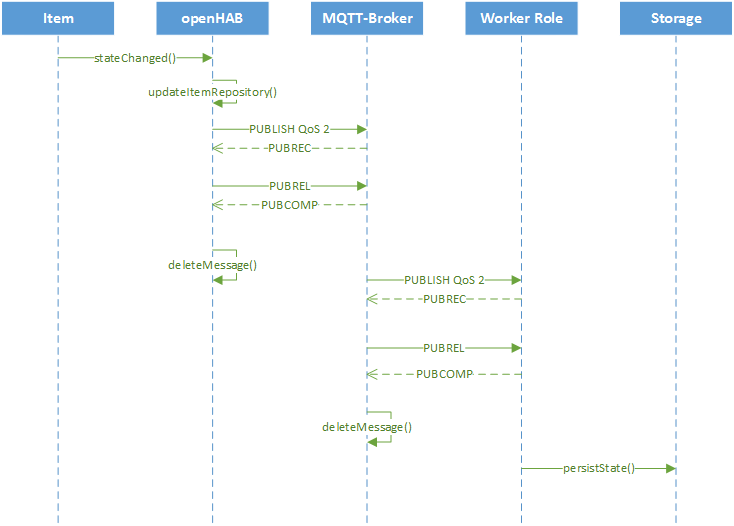
\includegraphics[scale=0.8]{report/img/sequenzDiagramMqtt}
	\caption{Sequenzdiagramm MQTT}
	\label{fig:sequenzMQTT}
\end{figure}

\subsection{Android App}
\subsubsection{Technologien}
\textbf{ReactiveX} \\
\tbd

\textbf{Retrofit} \\
\tbd

\textbf{OkHttp} \\
\tbd

\textbf{Butterknife} \\
\tbd

\subsubsection{Architektur}

\subsubsection{Material Design}

\subsection{Notification}
Der Mobile-Client wird durch Notifications benachrichtig, sobald der Alarm ausgelöst wird. Umgesetzt wird dies mithilfe des Google Cloud Messaging Dienstes.

\subsubsection{Cloud}
Um den GCM-Dienst nutzen zu können, muss zu erst in der Google Developer Console (\url{https://console.developers.google.com}) ein Projekt erstellt werden mit einer Cloud-Messaging-API. Für diese API kann ein Schlüssel erzeugt werden, der für das Versenden der Notification über die neu erstellte API benötigt wird.

Ausgelöst wird der ganze Vorgang durch die MQTT-Nachricht «alarm\_activated». Die Worker Role nimmt diese Nachricht entgegen und erzeugt eine Notification-Message:

\begin{lstlisting}[style=csharp, caption=Notification.cs - Notification Message]
{
  "registration_ids" : ["APA91bHun4MxP5egoKMwt2KZFBaFUH-1RYqx..."],
  "data" : {
  	"message" : "Alarm wurde ausgeloest!"
  }
}
\end{lstlisting}

Die Registration-Id bezeichnet den Client, der die Message erhalten soll. Dazu müssen sich die Clients zuvor bei GCM registrieren und erhalten dann die Id. Diese Message muss also für jeden Client einzeln über einen HTTP-Post gesendet werden. GCM weiss anhand des Id-Strings an welche Android-Clients er die Message weiterleiten soll.

Folgende Grafik stellt den Registrations-Vorgang dar:
\begin{figure}[H]
	\centering
		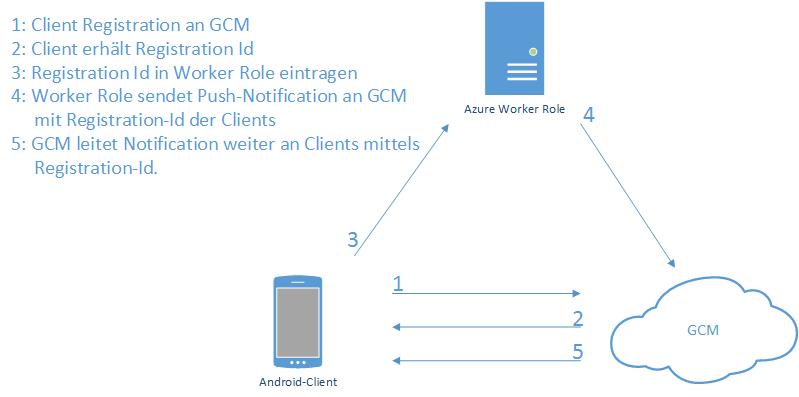
\includegraphics[scale=0.7]{report/img/gcm}
	\caption{Vorgang Push-Notification}
	\label{fig:notification}
\end{figure}

Die nachfolgende Grafik (Abbildung \ref{fig:sequenzNotification}) zeigt auf, wie anhand der MQTT-Message die Notifikation ausgelöst wird.

\begin{figure}[H]
	\centering
		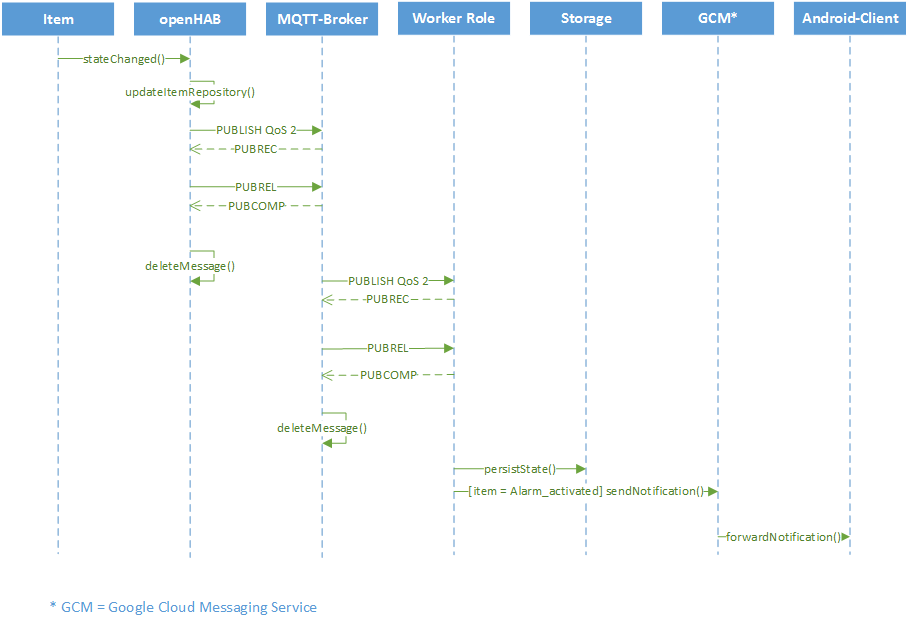
\includegraphics[scale=0.65]{report/img/sequenzDiagramNotification}
	\caption{Sequenzdiagramm MQTT-Notification}
	\label{fig:sequenzNotification}
\end{figure}

\subsubsection{Android-Client}


\subsection{Sicherheit}
Aus technischer Sicht können folgende Massnahmen getroffen werden, um die im Lösungskonzept beschriebenen Schwachstellen zu sichern:
\begin{itemize}
	\item Verschlüsselung der MQTT-Verbindung.
	\item Anmeldung am MQTT-Broker durch Benutzername \& Passwort.
	\item Verschlüsselung des WLANs.
\end{itemize}

\subsubsection{Verschlüsselung MQTT-Verbindung}
Die Verbindung zum MQTT-Broker wird durch SSL/TLS Verschlüsselt. Dazu wird ein Self-signed Zertifikat eingesetzt. Wie dieses Zertifikat erzeugt wird, ist aus dem Anhang \ref{ch:manual} zu entnehmen. \\
Die jeweilige Implementierung der TLS-Verbindung wird im Kapitel \ref{sssec:mqtt} erläutert.

\subsubsection{Konfiguration MQTT-Broker}
Am Broker sollen sich nur authentifizierte und autorisierte Clients anmelden können. Dazu bietet der MQTT-Standard die Möglichkeit ein Password-File zu erzeugen. In dieses File wird der Benutzername und das zugehörige Passwort eingetragen, mit dem sich die Clients anmelden können. Nur wenn diese Angaben übereinstimmen, kann eine Verbindung aufgebaut werden. \\
Mosquitto bringt ein Tool mit, zur Erzeugung und Verschlüsselung dieses Files. Über die Konsole wird das Skript aufgerufen und die Benutzerangaben können als Parameter übergeben werden:
\begin{lstlisting}[style=csharp, caption=mosquitto\_passwd.exe - generate password-file]
> mosquitto_passwd -c passwordFile
> mosquitto_passwd -b passwordFile username password
\end{lstlisting}
Wie sich die Clients gegenüber dem Broker authentifizieren, ist im Abschnitt \ref{sssec:m2mqttClient} und \tbd (MQTT Binding) ersichtlich.

\subsubsection{Verschlüsselung WLAN}
Über das WLAN kann man ohne Authentifizierung auf das openHAB zugreifen. Um unautorisierten Zugriff zu verhindern, wird das WLAN mit dem Sicherheitsstandard WPA2 verschlüsselt. Die Kommunikation wird also über den symmetrischen AES (Advanced Encryption Standard) Algorithmus verschlüsselt. Da es sich um eine symmetrische Verschlüsselung handelt, muss jeder Client ein PSK (Pre Shared Key) besitzen, der jeweils beim Verbindungsaufbau eingegeben werden muss.





